\documentclass[tikz]{standalone}
\usetikzlibrary{calc,through,intersections,backgrounds}
\begin{document}
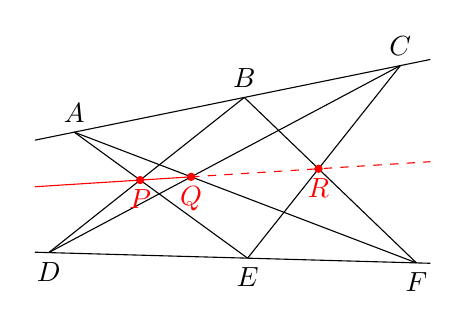
\begin{tikzpicture}
  % draw the given points first
  \coordinate [label=above:$A$] (A) at ($ (0.2,1.8) + .1*(rand,rand) $);
  \coordinate [label=above:$B$] (B) at ($ (2.3,2.2) + .1*(rand,rand) $);
  \draw (A) -- (B)
    -- ($ (A) ! 2+.1*rand ! (B) $) coordinate [label=above:$C$] (C);
  \coordinate [label=below:$D$] (D) at ($ (0,0.3) + .1*(rand,rand) $);
  \coordinate [label=below:$E$] (E) at ($ (2.5,0.2) + .1*(rand,rand) $);
  \draw (D) -- (E)
    -- ($ (D) ! 2+.3*rand ! (E) $) coordinate [label=below:$F$] (F);

  % set the visible area of the figure
  \clip
    let \p1=(A),
        \p2=(C),
        \p3=(D),
        \p4=(F),
	\n5={(min(\x1,\x2,\x3,\x4))-5},
	\n6={(min(\y1,\y2,\y3,\y4))-5},
	\n7={(max(\x1,\x2,\x3,\x4))+5},
	\n8={(max(\y1,\y2,\y3,\y4))+5}
    in
      (\n5,\n6) rectangle (\n7,\n8);

  % Extend the given segments so that they look like lines
  \draw (A) -- ($ (A) ! -1 ! (B) $);
  \draw (C) -- ($ (A) ! 3 ! (B) $);
  \draw (D) -- ($ (D) ! -1 ! (E) $);
  \draw (F) -- ($ (D) ! 3 ! (E) $);

  % Draw the segments
  \draw [name path=A--E] (A) -- (E);
  \draw [name path=B--D] (B) -- (D);
  \draw [name path=B--F] (B) -- (F);
  \draw [name path=C--E] (C) -- (E);
  \draw [name path=A--F] (A) -- (F);
  \draw [name path=C--D] (C) -- (D);

  % Get the intersection points
  \def\P{\textcolor{output}{$P$}}
  \def\Q{\textcolor{output}{$Q$}}
  \def\R{\textcolor{output}{$R$}}
  \colorlet{output}{red}

  \path [name intersections={of=A--E and B--D, by={[label={[label distance=0]-90:\P}]P}}];
  \path [name intersections={of=B--F and C--E, by={[label=below:\R]R}}];
  \path [name intersections={of=A--F and C--D, by={[label=below:\Q]Q}}];

  % Colour the intersection points
  \foreach \pt in {P,Q,R}
    \fill [output] (\pt) circle (1.5pt);

  % Point out the problem
  \draw [output] ($ (P) ! -5 ! (Q) $) -- (P) -- (Q);
  \draw [output,dashed] (Q) -- (R) -- ($ (P) ! 9 ! (Q) $);
\end{tikzpicture}
\end{document}
